\begin{figure}[h!]
	\center
	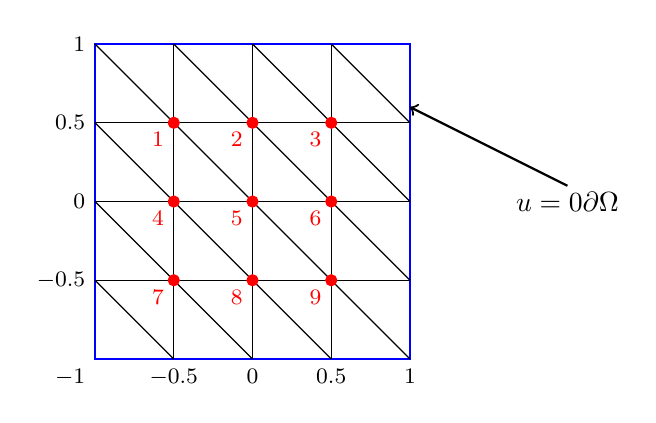
\begin{tikzpicture}[scale=2]
	
	\pgfmathsetmacro{\zerox}{-1}
	\pgfmathsetmacro{\zeroy}{-1}
	
	\draw[blue] (\zerox,\zeroy) -- ++(2,0)-- ++(0,2) --++(-2,0) --cycle;
	
	%vertical lines
	\draw (\zerox,\zeroy) ++(0.5,0)-- ++(0,2);
	\draw (\zerox,\zeroy) ++(1,0)-- ++(0,2);
	\draw (\zerox,\zeroy) ++(1.5,0)-- ++(0,2);
	
	% horizontal lines
	\draw (\zerox,\zeroy) ++(0,0.5)-- ++(2,0);
	\draw (\zerox,\zeroy) ++(0,1)-- ++(2,0);
	\draw (\zerox,\zeroy) ++(0,1.5)-- ++(2,0);
	
	% diagonal lines
	\draw (\zerox,\zeroy) ++(0,0.5)-- ++(0.5,-0.5);
	\draw (\zerox,\zeroy) ++(0,1)-- ++(1,-1);
	\draw (\zerox,\zeroy) ++(0,1.5)-- ++(1.5,-1.5);
	\draw (\zerox,\zeroy) ++(0,2)-- ++(2,-2);
	\draw (\zerox,\zeroy) ++(0.5,2)-- ++(1.5,-1.5);
	\draw (\zerox,\zeroy) ++(1,2)-- ++(1,-1);
	\draw (\zerox,\zeroy) ++(1.5,2)-- ++(0.5,-0.5);
	
	
	% inner points
	\filldraw[red]  (\zerox,\zeroy) ++ (0.5,0.5) circle (1pt)
					(\zerox,\zeroy) ++ (0.5,1) circle (1pt)
					(\zerox,\zeroy) ++ (0.5,1.5) circle (1pt)
					(\zerox,\zeroy) ++ (1,0.5) circle (1pt)
					(\zerox,\zeroy) ++ (1,1) circle (1pt)
					(\zerox,\zeroy) ++ (1,1.5) circle (1pt)
					(\zerox,\zeroy) ++ (1.5,0.5) circle (1pt)
					(\zerox,\zeroy) ++ (1.5,1) circle (1pt)
					(\zerox,\zeroy) ++ (1.5,1.5) circle (1pt);
	
	
	
	\fill[red,font=\footnotesize] (\zerox,\zeroy) ++ (0.5,1.5)  node[below left] {$1$}
								  (\zerox,\zeroy) ++ (1,1.5)  node[below left] {$2$}
								  (\zerox,\zeroy) ++ (1.5,1.5)  node[below left] {$3$}
								  (\zerox,\zeroy) ++ (0.5,1)  node[below left] {$4$}
								  (\zerox,\zeroy) ++ (1,1)  node[below left] {$5$}
								  (\zerox,\zeroy) ++ (1.5,1)  node[below left] {$6$}
								  (\zerox,\zeroy) ++ (0.5,0.5)  node[below left] {$7$}
								  (\zerox,\zeroy) ++ (1,0.5)  node[below left] {$8$}
								  (\zerox,\zeroy) ++ (1.5,0.5)  node[below left] {$9$};
	
	
	% axis numbering
	\fill[black,font=\footnotesize] (\zerox,\zeroy)  node[below left] {$-1$}
									(\zerox,\zeroy) ++(0.5,0) node[below] {$-0.5$}
									(\zerox,\zeroy) ++(1,0) node[below] {$0$}
									(\zerox,\zeroy) ++(1.5,0) node[below] {$0.5$}
									(\zerox,\zeroy) ++(2,0) node[below] {$1$}
									
									(\zerox,\zeroy) ++(0,0.5) node[left] {$-0.5$}
									(\zerox,\zeroy) ++(0,1) node[left] {$0$}
									(\zerox,\zeroy) ++(0,1.5) node[left] {$0.5$}
									(\zerox,\zeroy) ++(0,2) node[left] {$1$};
									
   	\node at (\zerox + 3,\zeroy + 1) {$u=0 \ton \partial \Omega$};
   	\draw[thick,-to] (\zerox + 3 ,\zeroy + 1.1) -- ++(-1,0.5);							    
	
	\end{tikzpicture}
		
	\caption{meshed $\Omega $}\label{tikz/chapter2/mesh_omega}
	\label{ch2_mesh_omega}

\end{figure}